% Default Compiler: txs:///xelatex | txs:///bibtex
% Default Bibliography Tool: BibTex

\documentclass[12pt,onecolumn,a4paper]{article}
\usepackage{listings}
\usepackage{epsfig,graphicx,subfigure,amsthm,amsmath}
\usepackage{caption}
%\usepackage{color}
\usepackage[table, svgnames, usenames,dvipsnames]{xcolor} \usepackage{array}
\usepackage{tabularx}
\usepackage{etoolbox}
\usepackage{cellspace}
\usepackage{float}
\usepackage{hhline}
\usepackage[linktocpage=true,colorlinks,citecolor=blue,pagebackref=true]{hyperref}
\usepackage[top=30mm, bottom=30mm, left=30mm, right=30mm]{geometry}
%\usepackage[T1]{fontenc}
\usepackage[utf8]{inputenc}
\usepackage{fontspec}
\setmainfont{Doulos SIL}
\usepackage{authblk}
\usepackage{polyglossia}
\setotherlanguage{english}
\setotherlanguage{persian}
\usepackage[nonamebreak]{natbib}
\usepackage{xepersian}
\settextfont[Scale=1.2]{IRLotus}
\defpersianfont\mfo[Scale=1.2]{IRLotus}
\setlatintextfont[Scale=1]{Doulos SIL}

\setcounter{Maxaffil}{0}
\renewcommand\Authands{ و }
\renewcommand\Authand{ و }
\renewcommand\Affilfont{\itshape\small}
\providecommand{\keywords}[1]{\textbf{\textit{کلیدواژه‌ها:}} #1}

\setlength\cellspacetoplimit{4pt}
\setlength\cellspacebottomlimit{4pt}
\colorlet{headercolour}{DarkSeaGreen!40}

\DefaultMathsDigits

\definecolor{customblue}{RGB}{235,241,245}
\definecolor{light-gray}{gray}{0.95}
\lstdefinestyle{C++Style}{%
backgroundcolor=\color{customblue},
breaklines=true,
basicstyle=\footnotesize\ttfamily,
keywordstyle=\color{blue},
commentstyle=\color{OliveGreen}\textit,
stringstyle=\color{red},
numbers=left,
numberstyle={\tiny\lr},
showspaces = false,
showstringspaces = false,
tabsize = 2,
frame=single,
xleftmargin=5pt,
xrightmargin=3pt,
language = C++,
aboveskip = 20pt,
rulecolor=\color{black},
captiondirection=RTL,
}

\lstnewenvironment{C++Code}[1][]
{%
\lstset{style=C++Style, #1}%
}{%
}

\def\lstlistingname{شبه‌کد}

\begin{document}
    \title{بررسی آماری تحول زایایی وندهای اشتقاقی در نظم فارسی\footnote{هشتمین همایش زبان‌شناسی ایران، دانشگاه علامه طباطبائی، بهمن 1391}}
    \author[1]{وحید مواجی}
    \author[2]{محرم اسلامی}
    \affil[1]{دانشگاه صنعتی شریف}
    \affil[2]{دانشگاه زنجان}
    \date{24 بهمن 1391}
    \maketitle

    \begin{abstract}
        زایایی یکی از ویژگی‌های دستگاه صرف است که مشخص‌ترین خصوصیتش نسبی بودن آن است. یعنی یک فرایند واژه‌سازی در طول زمان می‌تواند زایایی خود را از دست بدهد یا اینکه زایاتر شود. از طرفی بین فرایندهای مختلف واژه‌سازی نیز زایایی نسبی است. زایایی ویژگی طیفی دارد که مقادیر آن می‌تواند در فرایندهای واژه‌سازی بین صفر (کاملاً سترون) و 1 (بسیار زایا) در نوسان باشد. با دو رویکرد می‌توان به مسأله زایایی نگریست: رویکرد هم‌زمانی و رویکرد درزمانی. در این مقاله از هر دو دیدگاه به مسأله نگریسته شده و با ارائه فرمول‌های ریاضی و محاسبات آماری روی پیکره‌ای از شعر فارسی (پیکره گنجور) با بیش از یک میلیون مصراع، زایایی فرایند اشتقاق پسوندی در نظم فارسی بررسی شده‌ است. این پیکره اشعار 52 شاعر فارسی‌زبان از قرن چهارم تا قرن چهاردهم هجری را شامل می‌شود. البته ممکن است تحلیل آماری منابع منظوم و نتایج به‌دست آمده از آن نمایندهٔ صددرصد زبان رایج مردم در دوره‌ای از تاریخ یک زبان نباشد، ولی حداقل بازتاب‌دهندهٔ بخشی از ویژگی‌های ساخت‌واژی در گونهٔ ادبی دوره‌های مختلف زبان فارسی خواهد بود. در این مقاله معیارهای مختلفی که برای سنجش میزان زایایی ارائه شده، مورد بررسی قرار گرفته است و با استفاده از روش تعداد تک‌وقوع‌ها و نیز تجزیهٔ خودکار کلمات به کمک یک تحلیل‌گر صرفی (پارس‌مورف)، میزان زایایی پسوندهای اشتقاقی از نظر درزمانی و هم‌زمانی با شاخص‌های عددی و آماری نشان داده می‌شود
        \par
        \keywords{واژه‌سازی، اشتقاق، زایایی درزمانی، زایایی هم‌زمانی، نظم فارسی}
    \end{abstract}

    \section{مقدمه}
    زایایی در صرف یکی از مسائل محوری مطالعات واژه‌سازی است و دیدگاه‌های مختلفی در بحث زایایی مطرح است. به اعتقاد \Latincite{bauer_2001}:
    \par\noindent
    الف) وندها زایا هستند؛ یعنی زایایی، ویژگی یک وند برای ساختن کلمات پیچیدهٔ جدید است \Latincite{plag_2003, fleischer_1975}.
    \par\noindent
    ب) فرایندهای صرفی زایا هستند یعنی ویژگی یک فرایند صرفی برای تشکیل سازه‌های جدید طبق اصول نظام‌مند، زایایی نام دارد \Latincite{uhlenbeck_78, anderson_1982}.
    \par\noindent
    علی‌رغم این که در بین مقالات بر سر این که چه چیزی زایا است، اختلاف وجود دارد، مطالعه کمّیِ زایایی بیشتر حول محور زایاییِ وند متمرکز شده است. معیارهای کمّیِ مختلفی برای سنجش زایایی ارائه شده است که برخی زایاییِ گذشته و برخی زایایی بالقوه را ارزیابی می‌کنند. باید توجه داشت که زایایی یک پدیده درزمانی است، بدین معنی که یک وند خاص ممکن است در زمان گذشته بسیار زایا بوده باشد مانند پسوند /-ak/ در زبان فارسی، ولی امروزه به ندرت کلمات جدیدی با این پسوند ساخته می‌شوند و لذا این پسوند غیرزایا می‌باشد {\mfo\citep{taba_82}}.

    \par
    در این پژوهش با بررسی‌های آماری روی پیکره‌ای نسبتاً غنی از نظم فارسی\footnote{پیکره گنجور} با بیش از یک میلیون مصراع شعر، تحول ساخت‌واژی زبان فارسی را در گونهٔ زبانی نظم و شعر مطالعه می‌کنیم. زبان شعر شاید نمایندهٔ زبان رایج مردم در دوره‌ای از تاریخ نباشد، ولی تحلیل آماری زایایی وندهای اشتقاقی در نظم و نتایج به‌دست‌آمده می‌تواند حداقل نشان‌دهندۀ بخشی از ویژگی‌های صرفی زبان فارسی در گونهٔ ادبی به عنوان تنها آثار باقیمانده از زبان فارسی باشد. شایان ذکر است که آثار منثور فارسی نیز نمایندهٔ تمام‌کمال زبان فارسی رایج در دوره‌ای از تاریخ ایران زمین نمی‌تواند باشد.

    \par
    یکی از مواردی که می‌توان روی این پیکره بررسی کرد، بحث زایایی فرایندهای واژه‌سازی در زبان فارسی است. این بررسی را می‌توان از دو منظر مورد توجه قرارداد: از دید هم‌زمانی یعنی زایایی نسبی فرایندهای واژه‌سازی در یک بازه زمانی از تاریخ و از دید درزمانی یعنی تحول زایایی یک فرایند واژه‌سازی در طول زمان. فرایندهای واژه‌سازی در فارسی شامل ترکیب و اشتقاق می‌باشد که در این مقاله، فرایند اشتقاق پسوندی در زبان فارسی مورد بررسی قرار می‌گیرد.

    \par
    بحث اینکه چه معیاری برای سنجش زایایی مناسب می‌باشد بحث گسترده‌ای است. در این مقاله معیارهای مختلفی که برای سنجش میزان زایایی ارائه شده است مورد بررسی قرار گرفته و با استفاده از روش تعداد تک‌وقوع‌ها\LTRfootnote{\lr{Hapaxes}} معیاری عددی و آماری برای سنجش میزان زایایی وندهای اشتقاقی ارائه می‌شود و نتایج بدست آمده از دید درزمانی و هم‌زمانی ارائه می‌گردد.

    \section{معیارهای زایایی صرفی}
    در ادامه به معرفی مدل‎های ارزیابی زایایی می‌پردازیم.

    \subsection{مدل آرونوف}
    \Latincite{aronoff_1976}، به نقل از بائر \Latincite{bauer_2001}، نسبتِ کلمات بالفعلِ ساخته شده در چارچوب یک قاعده واژه‌سازی \lr{(WFR\LTRfootnote{\lr{Word-Formation Rule}})} را به کلمات بالقوۀ قابل تولید از آن قاعده، طبق فرمول زیر محاسبه می‌کند:
    \begin{equation}
        I=v / s
    \end{equation}
    که در آن $I$ شاخص زایایی است؛ $v$ تعداد نوع‌کلمه‌های واقعی است، و $s$ تعداد نوع‌کلمه‌هایی است که WFR می‌تواند تولید کند.

    \subsection{مدل‌های بسامدی}
    مدل‌های بسامدی روی این فرض استوار هستند که بسامد به طور مستقیم یا غیرمستقیم با زایایی مرتبط است. منظور از «بسامد» تعداد دفعات وقوع یک کلمه در یک پیکره است. در خصوص موضوع بسامد سه نظر مختلف مطرح است که در آنها به ترتیب بسامد نوع‌\LTRfootnote{\lr{Type}}، بسامد نمونه\LTRfootnote{\lr{Token}} و بسامد نسبی مد نظر می‌باشد. به عنوان مثال اگر 100 کلمه با پسوند /-ande/ در یک پیکرهٔ زبانی فارسی باشد برای مثال در «گوینده، جوینده، کشنده»، می‌گوییم بسامد نوع برابر 100 است. بسامد نمونه در همین پیکرهٔ زبانی ممکن است بیش از 100 باشد، چراکه ممکن است هر کدام از آن 100 کلمه بیش از یک بار تکرار شده باشد.

    \subsubsection{بسامد نوع}
    یک دیدگاه این است که وندی زایاتر است که تعداد کلمات زیادی با استفاده از آن ساخته شده باشد. بنابراین یکی از پرکاربردترین معیارها در مقالات، شمارش سادۀ تعداد نوع‌کلمه‌های بالفعل ساخته شده با آن وند در یک دورۀ زمانی خاص است. البته این معیار به همان اندازه هم مورد مخالفت قرار گرفته است به این دلیل که یک وند ممکن است در گذشته کلمات زیادی را می‌ساخته ولی امروزه گویشوران زبان به ندرت کلمه جدیدی را از رهگذر آن می‌سازند. مثال چنین وندی، «-اک» در فارسی یا «-ment» در انگلیسی می‌باشد که در قرون گذشته کلمات جدید زیادی با آن ساخته می‌شده و بسیاری از آن کلمات هنوز به کار می‌روند ولی در حال حاضر کلمه جدیدی با آنها ساخته نمی‌شود و غیرزایا به شمار می‌روند \Latincite{plag_2003}.

    \subsubsection{بسامد نمونه}
    از آنجا که بسامد نوع‌ دارای مشکلاتی در ارزیابی زایایی است، یک راهکار دیگر برای بررسی زایایی، محاسبه بسامد نمونه است. \Latincite{baayen_1993} رابطه بین بسامد و زایایی را مورد بررسی قرار داده است. طبق این نظر، یک فرایند صرفی زایا متناظر تعداد زیادی کلمۀ کم‌بسامد و تعداد اندکی کلمه پربسامد است، در حالی که فرایندهای غیرزایا متناظر تعداد زیادی کلمۀ پربسامد و تعداد اندکی کلمه کم‌بسامد می‌باشند. منطق پشت این قضیه این است که کلمات مرکب پربسامد به صورت یک کلمۀ واحد در واژگان ذهنی ذخیره می‌شوند و کلمات مرکب کم‌بسامد به صورت سازه‌های تشکیل‌دهندۀ آنها در واژگان ذهنی ذخیره می‌شوند. دلیل این که یک کلمه مرکب تازه ساخته شده \rl{(مثلاً \lr{dis-represent})} برای گویشورانی که قبلاً هیچ وقت آن را نشنیده‌اند قابل فهم است، این است که آنها این کلمه را به سازه‌های تشکیل دهنده‌اش تجزیه می‌کنند، معنی تکواژهای سازنده را استنباط کرده و سپس معنی کل کلمه را ادراک می‌کنند.
    \par
    در حقیقت باید بین بسامد نوع‌ با بسامد نمونه تمایز قائل می‌شویم \Latincite{booij_2007}. بسامد نمونه شامل همهٔ کلمات پیچیدهٔ حاصل یک قاعدهٔ واژه‌سازی و نیز شامل کل وقوع‌های یک کلمه با تمامی شکل‌هایش می‌باشد. همانطور که پیشتر گفتیم، مثلاً اگر 100 صفت مختلف داشته باشیم که به «-وار» ختم شده باشند، بسامد نوع‌کلمه این پسوند برابر 100 است ولی بسامد نمونه آن می‌تواند بسیار بیشتر از این باشد، چون هر یک از این صفت‌ها خود می‌توانند به دفعات در متن مورد مطالعه تکرار شوند.
    \par
    بسامد نوع‌کلمه را در یک پیکره نسبتاً بزرگ باید محاسبه کرد نه لغتنامه یا دایره‌المعارف. زایایی صرفی در بهترین حالت، خود را در ساختن کلماتی نشان می‌دهد که در لغتنامه وارد نشده‌اند، چون یک کلمه جدید وقتی ساخته می‌شود مدت زمانی باید صرف شود تا این کلمه تثبیت شود و بعد از مدتی وارد لغتنامه ‌شود یا در مورد برخی کلمات شاید هیچ وقت وارد لغتنامه نشوند. بنابراین یک پیکره معیار مناسبتری است. با این حال، بسامد نوع‌کلمه حتی در یک پیکره بزرگ هم معیار خوبی برای زایایی بدست نمی‌دهد، زیرا زایایی به معنی قابلیت ساختن کلمات جدید است، کلماتی که هنوز وجود ندارند.

    \subsubsection{بسامد نسبی}
    بسامد نسبی، بسامد پایه‌های مشتق‌شده و واژگانی را با هم در نظر می‌گیرد، با این فرض که یک فرایند زایاتر است اگر بسامد پایه‌های مشتق‌شده کمتر از بسامد پایه‌های واژگانی باشد و در غیر این‌صورت زایایی آن کمتر است. در این معیار، بسامد پایه‌های مشتق‌شده بر بسامد پایه‌های واژگانی تقسیم می‌شود. هر چه عدد حاصله بالاتر باشد، آن وند یا فرایند کمتر زایاست.

    \subsection{مدل احتمالاتی}
    مدل‌های احتمالاتی عمدتاً توسط باین \Latincite{baayen_1989,baayen_1991,baayen_1992} ارائه شده‌اند. مجموعه این مدل‌ها به صورت آماری، احتمال وقوع یک کلمه جدید در قالب یک فرایند ساخت‌واژی را محاسبه می‌کنند. در مدل‌های احتمالاتی، محاسبه زایایی ناگزیر مستلزم در نظر گرفتن تک‌وقوع‌ها است. تک‌وقوع‌ها کلماتی هستند که تنها یک بار در پیکره رخ می‌دهند. طبق نظر باین، اگر بخواهیم زایایی را مطالعه کنیم باید تک‌وقوع‌ها را مورد بررسی قرار دهیم. بنابراین می‌توان میزان زایایی یک فرایند صرفی یا $P$ را بدین صورت تعریف نمود \Latincite{baayen_1992}:

    \begin{equation}
        P = n1 / N\label{eq:2}
    \end{equation}

    که $n1$ تعداد تک‌وقوع‌های نوع کلمه و $N$ تعداد کل وقوع‌های آن نوع کلمه (نمونه) در پیکره می‌باشد. در این مقاله ما از همین روش برای محاسبه زایایی وندهای مختلف در نظم فارسی استفاده خواهیم کرد.

    \section{منابع نظم فارسی}
    منابع مورد نظر از پروژه گنجور\LTRfootnote{\lr{http://ganjoor.net }}  استخراج شده است. این پروژه به صورت متن‌آزاد و داوطلبانه انجام می‌شود و در زمان نگارش این مقاله شامل اشعار 52 شاعر فارسی‌زبان از قرن چهارم تا قرن چهاردهم می‌باشد. این پروژه برای ذخیره دادگان خود از فرمت پایگاه داده Sqlite بهره می‌برد.
    \par\noindent
    جداول دادگان گنجور بدین شرح می‌باشند:
    \begin{itemize}
        \item جدول \lr{Poet}: این جدول اطلاعات شاعران را نگهداری کرده و شامل ویژگی‌های نام شاعر، قرن شاعر مربوطه و شرح مختصری از زندگی شاعر است.
        \item جدول \lr{Category}: این جدول نقش مقوله بندی شعرا و شعرها را دارد.
        \item جدول \lr{Poem}: این جدول اطلاعات شعرها را نگه‌داری می‌کند (مثلاً یک غزل از حافظ یا یک حکایت از سعدی).
        \item جدول \lr{Verse}: این جدول که اصلی‌ترین جدول می‌باشد، اطلاعات تک مصراع‌ها را در خود دارد.
    \end{itemize}
    \par
    ارتباط این جدول‌ها با هم و نمودار UML آنها در شکل \ref{fig:1} آمده است.

    \begin{figure}[H]
        \centering
        \makebox[\textwidth]{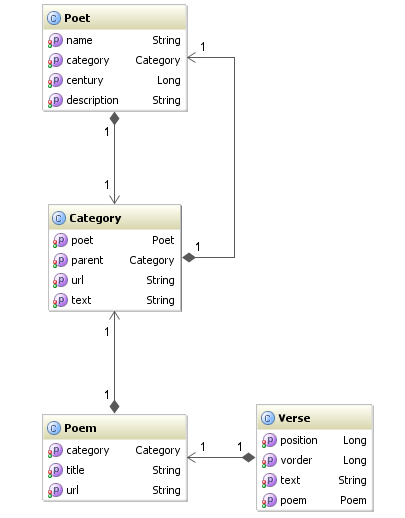
\includegraphics[scale=0.5]{icl1.png}}
        \caption{ ارتباط جداول موجود در پایگاه داده گنجور}
        \label{fig:1}
    \end{figure}
    \par
    جدول Poet شامل 52 سطر، جدول Category شامل 612 سطر، جدول Poem شامل 38742 سطر و جدول Verse شامل 1067292 سطر می‌باشند که منبعی غنی برای تحلیل آماری نظم فارسی را در اختیار ما می‌گذارند.

    \section{الگوریتم به‌کاررفته}
    برای بررسی وندها، از دادگان زایا یا FLexicon \citep{eslami_83} استفاده گردید. این دادگان دارای جدولی به نام Affix می‌باشد که شامل 170 وند است و از این تعداد 83 وند اشتقاقی داریم که در حقیقت پسوند می‌باشند.  الگوریتم به‌کاررفته، تک‌تک وندهای اشتقاقی را با استفاده از تحلیلگر صرفی پارس‌مورف \citep{mavaji_90} روی اشعار شاعران مختلف پیدا کرده و با استفاده از فرمول \ref{eq:2} زایایی آنها را محاسبه می‌کند. به علت تعدد وندها و شاعران، نتایج بسیار زیادی به‌دست آمد که برای داشتن یک دید درزمانی، این نتایج بر حسب قرن طبقه‌بندی گردید. مثلاً زایایی وند  «-کده» در قرن چهارم الی چهاردهم به چه نحوی بوده است. بنابراین 83 نمودار درزمانی بدست می‌آید که تحول زایایی این وندها را طی 10 قرن به‌دست می‌دهند. از طرفی 10 نمودار هم‌زمانی مربوط به هر قرن به‌دست آمد که زایایی 83 وند در هر کدام از قرن‌ها را نشان می‌دهد. مسأله‌ای که وجود داشت این بود که توزیع کمّیِ شعرها برای قرن‌های مختلف برابر و یکسان نبود. لذا با استفاده از تقریب مهندسی و مقیاس‌گذاری\LTRfootnote{\lr{Scaling}} دادگان، سعی گردید تا حد امکان نمودارهایی هموار\LTRfootnote{\lr{Smooth}} بدست آید.

    \section{نتایج به‌دست‌آمده}
    همانطور که در بخش قبل گفته شد، دو نوع نمودار بدست آمد:
    \begin{itemize}
        \item 10 نمودار هم‌زمانی برای هر یک از 10 قرن که در آنها زایایی هرکدام از 83 پسوند اشتقاقی آمده است.
        \item 83 نمودار در زمانی که در هر کدام از آنها تحول زایایی یک پسوند اشتقاقی خاص در طی 10 قرن نشان داده شده است.
    \end{itemize}

    برای مثال نمودار هم‌زمانی زایایی وندها برای قرن هفتم در شکل \ref{fig:2} آمده است. همانطور که از نمودار مشخص است وندهایی مانند: «-آگین»، «-ابر»، «-جو»، «-دیس» و «-ساز» دارای بیشترین زایایی و وندهایی مثل «-سیر»، «-گر»، «-گسار» و «-واره» دارای کمترین زایایی در قرن هفتم بوده‌اند. وندهایی هم مثل «-گرا»، «-گون»، «-پذیر» و «-خواه» دارای زایایی بینابینی بوده‌اند.

    \begin{figure}[H]
        \centering
        \makebox[\textwidth]{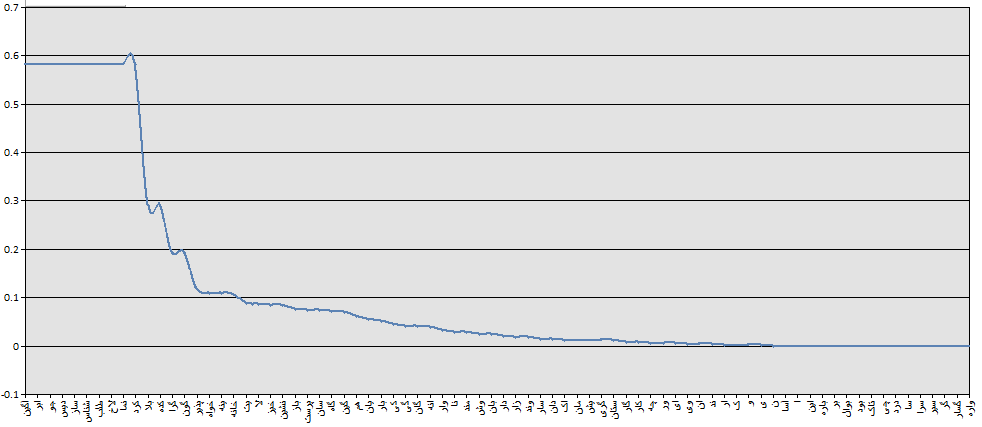
\includegraphics[width=\textwidth]{icl2.png}}
        \caption{نمودار هم‌زمانی زایایی وندها در قرن هفتم (محور افقی، وندها و محور عمودی میزان زایایی را نشان می‌دهد)}
        \label{fig:2}
    \end{figure}

    در شکل \ref{fig:3}، مثالی از نمودار درزمانی تحول زایایی وندها برای وند «-ار»  آورده شده است (محور افقی نشان‌دهنده قرن و محور عمودی میزان زایایی را نشان می‌دهد). همانطور که دیده می‌شود و در بخش‌های قبلی این مقاله نیز ذکر گردید، زایایی وندها مقدار ثابتی نیست و با گذشت زمان ممکن است کمتر یا بیشتر گردد. مثلاً در قرن ششم، این وند نسبتاً زایا بوده تا اینکه در قرن نهم به کمترین میزان زایایی خود رسیده و باز روند افزایش تا قرن دوازدهم داشته و در قرن سیزدهم زایایی آن کمتر شده و در قرن چهاردهم به بیشترین میزان زایایی خود رسیده است. البته باید توجه داشت که تمام این نتایج روی متون نظم فارسی گرفته شده است و اگر روی پیکره‌های دیگر مثل روزنامه‌ها، مجلات متون منثور و کتب بررسی شود، ممکن است نتایج متفاوتی بدست آید. نمودار مشابهی هم برای وند «-کده» به منظور مقایسه در شکل \ref{fig:4} آورده شده است.

    \begin{figure}[H]
        \centering
        \makebox[\textwidth]{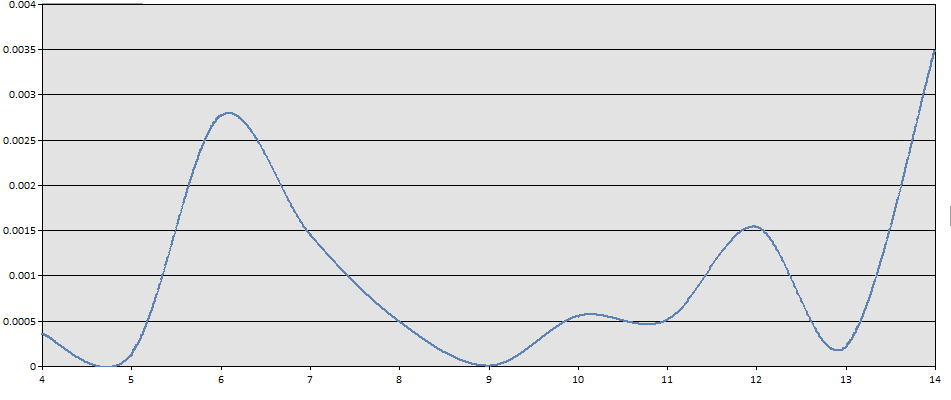
\includegraphics[width=\textwidth]{icl3.png}}
        \caption{نمودار درزمانی زایایی وند «-ار» در طی قرن 4 الی 14}
        \label{fig:3}
    \end{figure}

    \begin{figure}[H]
        \centering
        \makebox[\textwidth]{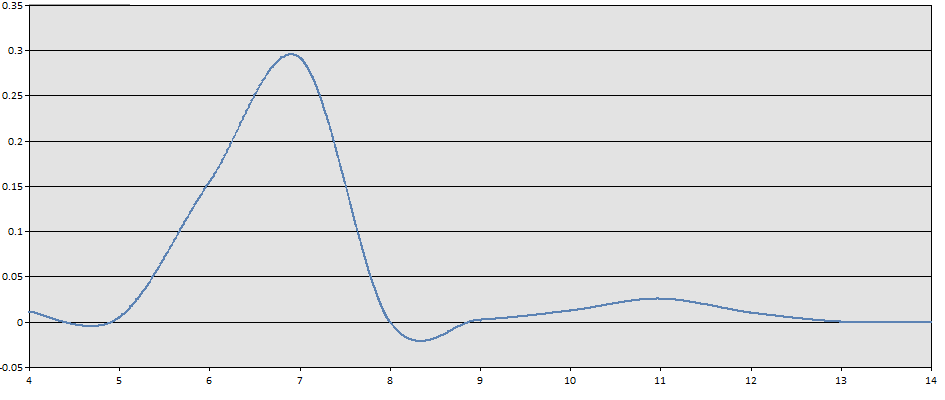
\includegraphics[width=\textwidth]{icl4.png}}
        \caption{نمودار درزمانی زایایی وند «-کده» در طی قرن 4 الی 14}
        \label{fig:4}
    \end{figure}

    \section{نتیجه‌گیری}
    در این تحقیق کوشیده‌ایم موضوع زایایی را در حوزهٔ اشتقاق پسوندی به عنوان بخشی از ویژگی‌های ساخت‌واژی زبان فارسی مورد مطالعه قرار دهیم. در تحقیق حاضر، مسألهٔ زایایی متناسب با طبیعت موضوع به دو صورت درزمانی و هم‌زمانی مورد بررسی قرار گرفته که در آن حیات 83 پسوند فارسی در 10 قرن جداگانه ترسیم شده است که به دلیل محدودیت در حجم مقاله تنها به ارائهٔ چند نمونه اکتفا کرده‌ایم. بررسی پیکرهٔ عظیم گنجور که برخودار از بیش از یک میلیون مصراع دادهٔ منظوم است می‌تواند بستر مناسبی را برای مطالعهٔ زایایی در در اختیار ما بگذارد و به دلیل گستردگی داده‌ها نتایج نیز از اعتبار و روایی لازم برخوردار باشد.
    \par
    از نتایج این تحقیق می‌توان در شناخت مسیر تحول زبان فارسی به طور عام و تحول در حوزهٔ ساخت‌واژه به طور خاص در مطالعات تاریخی و نیز رده‌شناختی استفاده کرد. مقایسهٔ دو فرایند عمدهٔ واژه‌سازی ترکیب و اشتقاق در 10 قرن می‌تواند گرایش‌های زبان فارسی را از نظر ساخت‌واژی روشن کند که به لحاظ نظری و کاربردی در امر واژه‌سازی و واژه‌گزینی حائز اهمیت است. همچنین نتایج این پژوهش شاید بتواند گوشه‌ای از تاریخ اجتماعی این مرزبوم را در معنای واژگانی که در این 10 قرن ساخته شده‌اند روشن کند که واژه‌های ساخته‌شده در هر دوره اشاره به باورها، مناسبات‌ زیست‌اجتماعی، ابزارهای تولید، عناوین در سلسله‌مراتب طبقات اجتماعی و غیره دارند.

    {\mfo
    \bibliographystyle{asa-fa}
    \bibliography{references}}

\end{document}